Les différents projets utilisant AIKON possèdent leur propre interface avec des bases de données distinctes hébergés sur des serveurs différents. Cependant, son aspect et son fonctionnement restent les mêmes.

\begin{figure}[h]
	\centering
	\begin{subfigure}{0.48\linewidth}
		\centering
		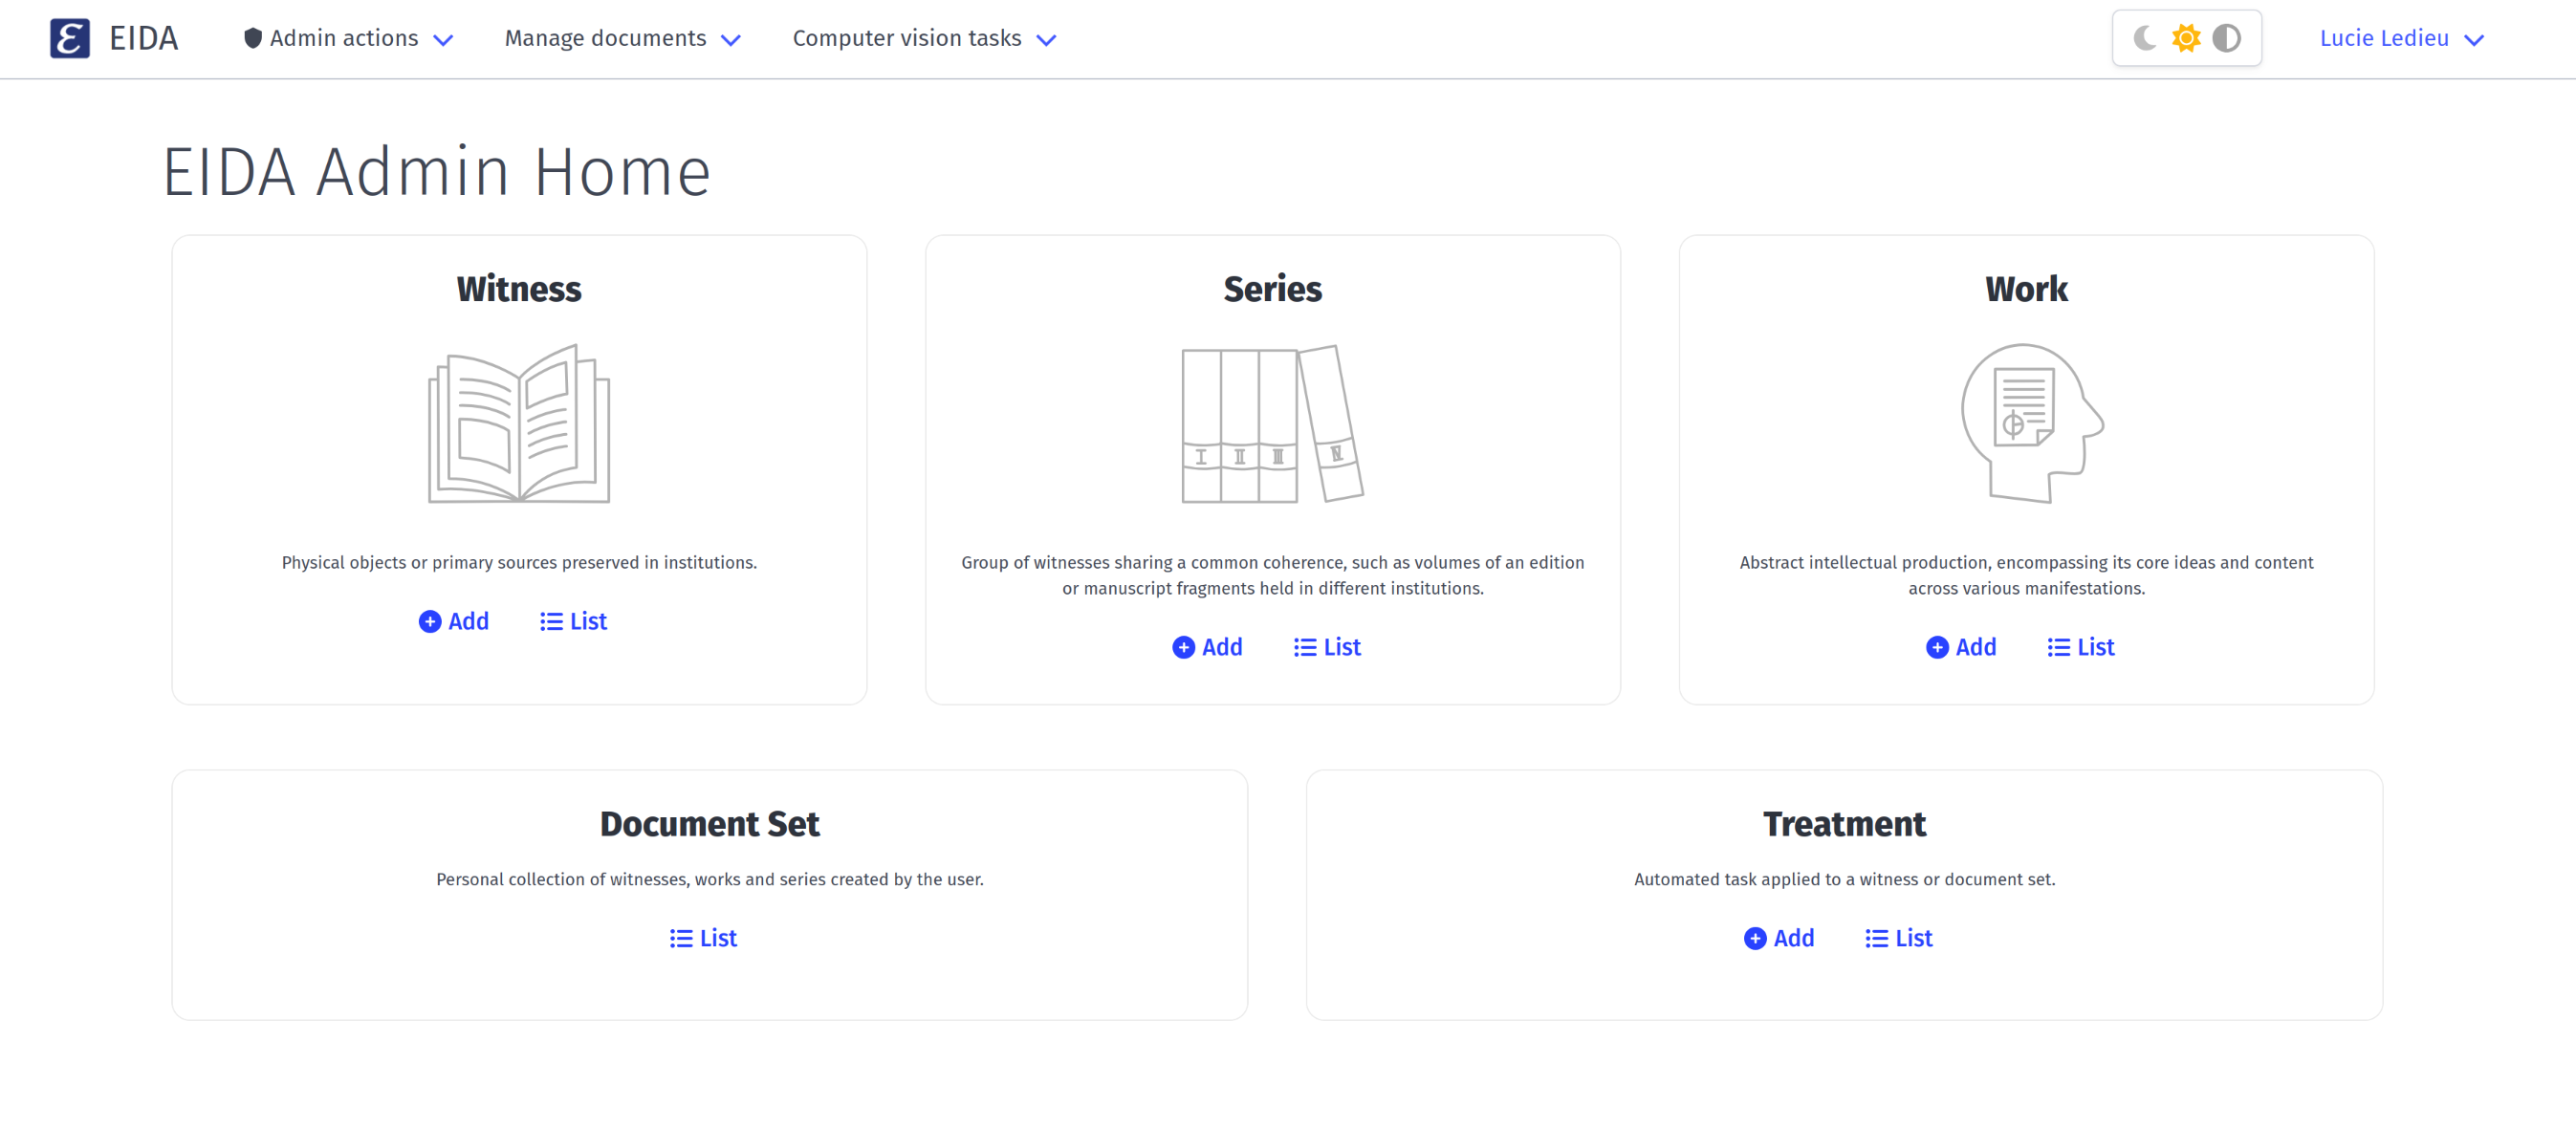
\includegraphics[width=\linewidth]{images/accueil_eida.png}
	\end{subfigure}
	\hfill
	\begin{subfigure}{0.48\linewidth}
		\centering
		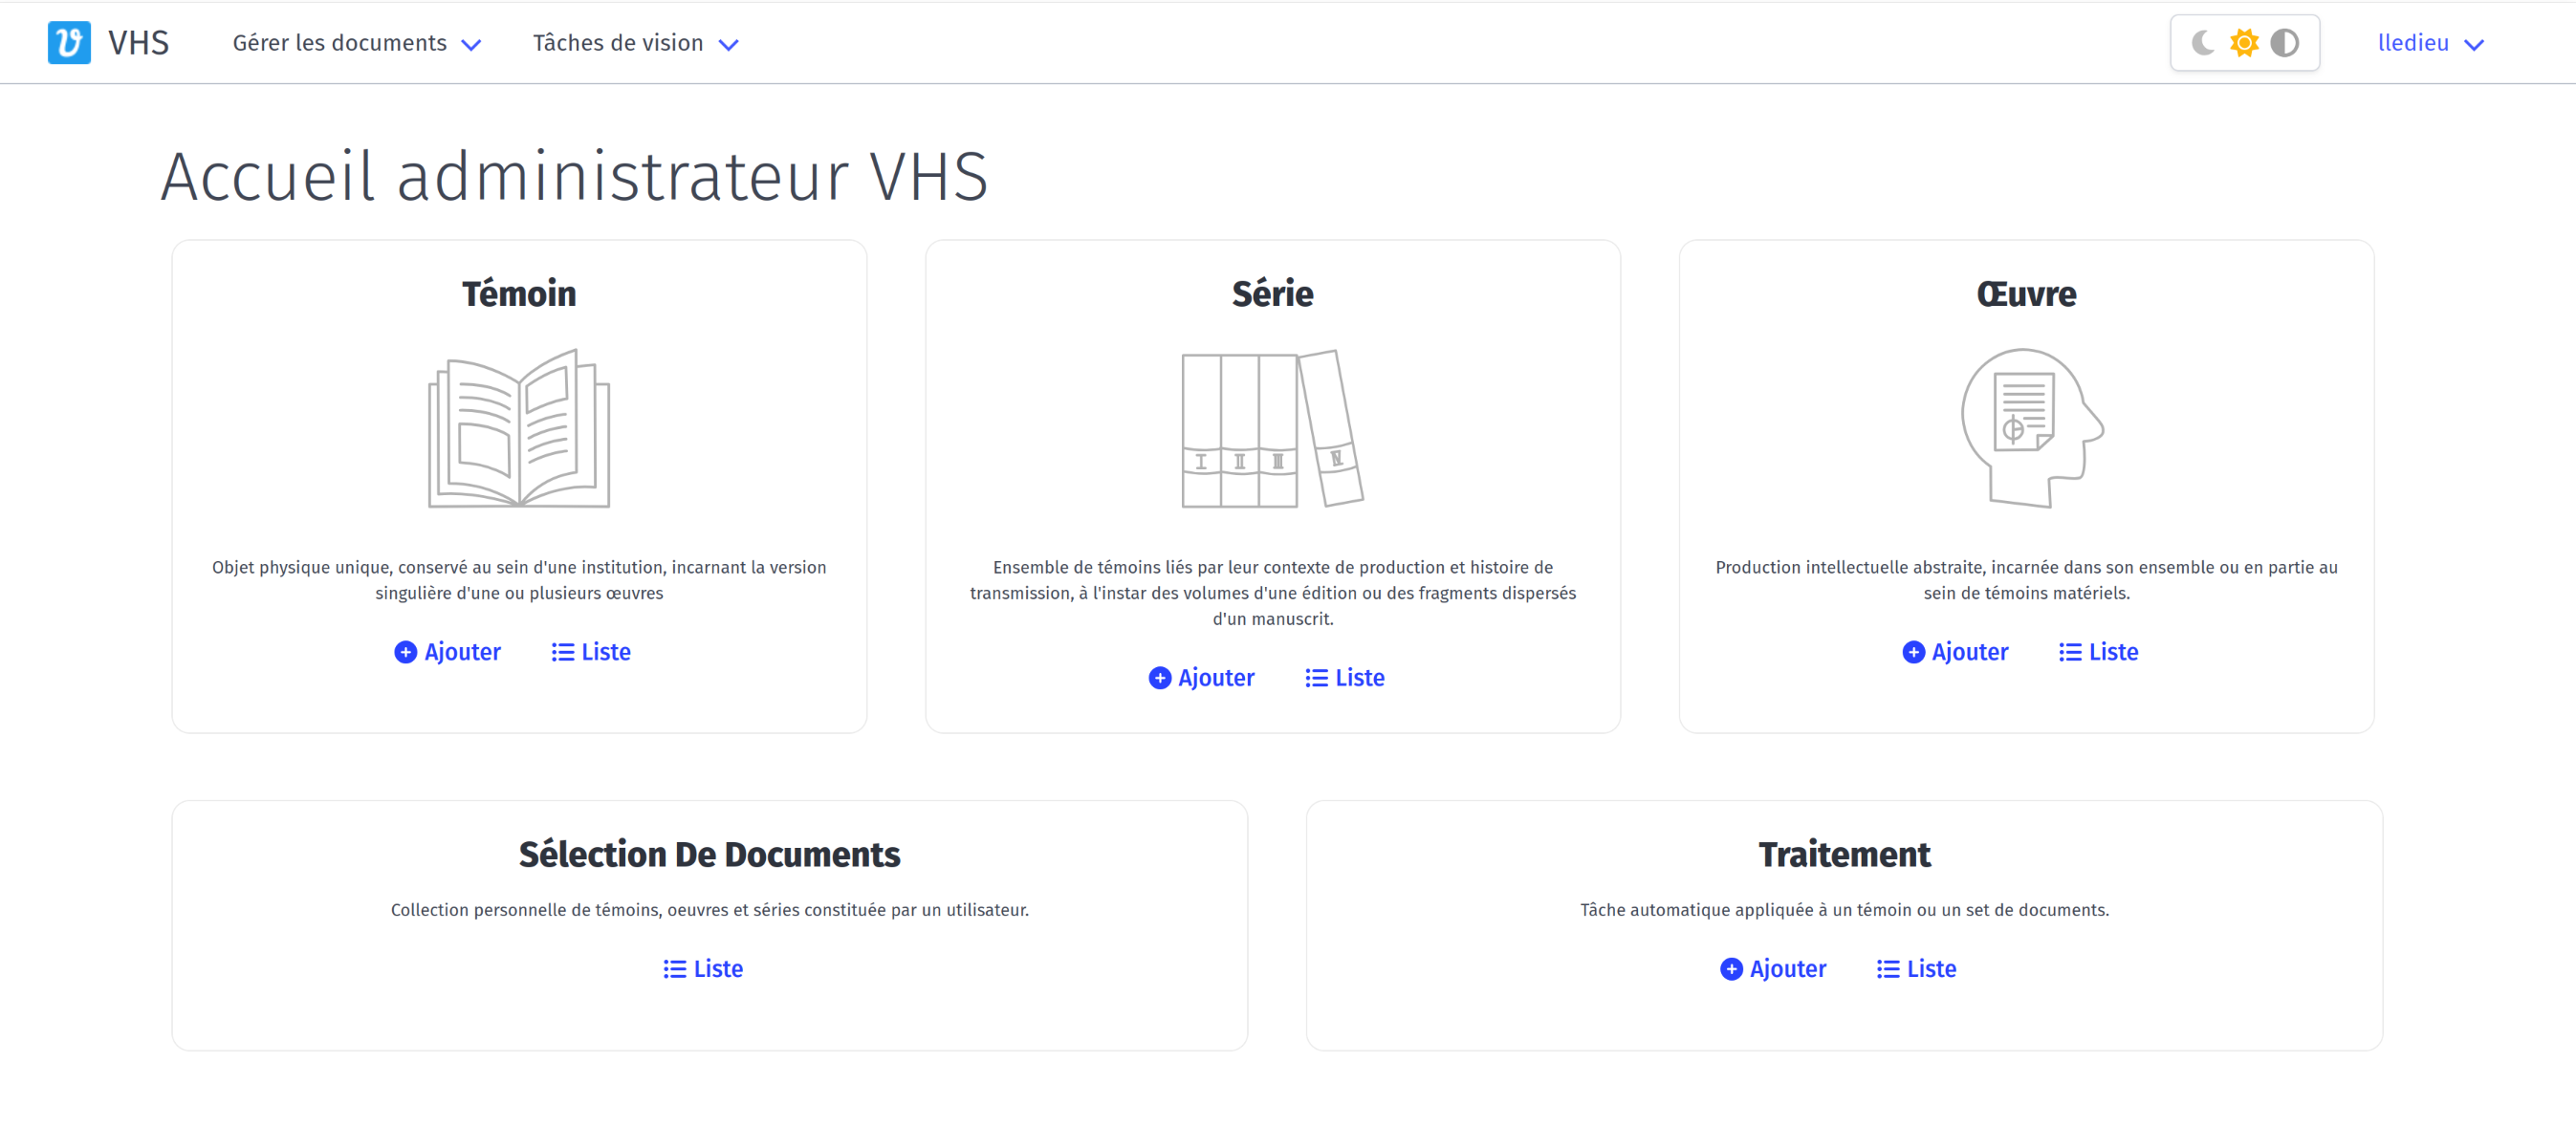
\includegraphics[width=\linewidth]{images/accueil_vhs.png}
	\end{subfigure}
	\caption{Interfaces administrateur EIDA et VHS}
	\label{fig:interface_accueil}
\end{figure}

Pour l'instant, ni \gls{vhs}, ni \gls{eida} ne possède d'interface publique. Les chercheurs utilisent actuellement l'interface administrateur, c'est-à-dire le \textit{back-office}. Ils possèdent chacun un compte avec un statut \og admin \fg tandis que les ingénieurs en charge du développement et de la gestion de l'application sont en mode \og super-admin \fg. L'avantage de ces interfaces est qu'il n'est pas nécessaire de savoir coder ou faire des requêtes \gls{sql}.

Un \textit{User's guide} détaillant les différentes options a été rédigé. Nous nous concentrerons sur les principales fonctionnalités.




\subsection{La constitution du corpus : gestion des sources numérisées}

Avant d'effectuer des traitements automatiques, l'application AIKON permet de constituer un corpus, le gérer et le partager. 

Pour ajouter la numérisation d'un document comme un manuscrit par exemple, il faut ajouter un nouveau  \textit{witness}. Il est possible de renseigner énormément de métadonnées pour le décrire comme sa cote, son lieu de conservation ou son type de pagination par exemple. Pour certaines catégories, comme c'est le cas avec le lieu de conservation, si celui de notre document n'est pas déjà disponible dans la base de données, nous devons le créer. Il pourra alors être réutilisé par les autres utilisateurs par la suite. En ce qui concerne le format de la numérisation, AIKON accepte les pdf, les manifestes \gls{iiif} ainsi que les images en format jpg ou png. 

Une fois le \textit{witness} ajouté à la base de données, les autres chercheurs inscrits sur la plateforme pourront accéder à lui et aux résultats des différents traitements qui lui seront appliqués. Un formulaire est d'ailleurs disponible pour affiner ses recherches.

\begin{figure}[H]
	\centering
	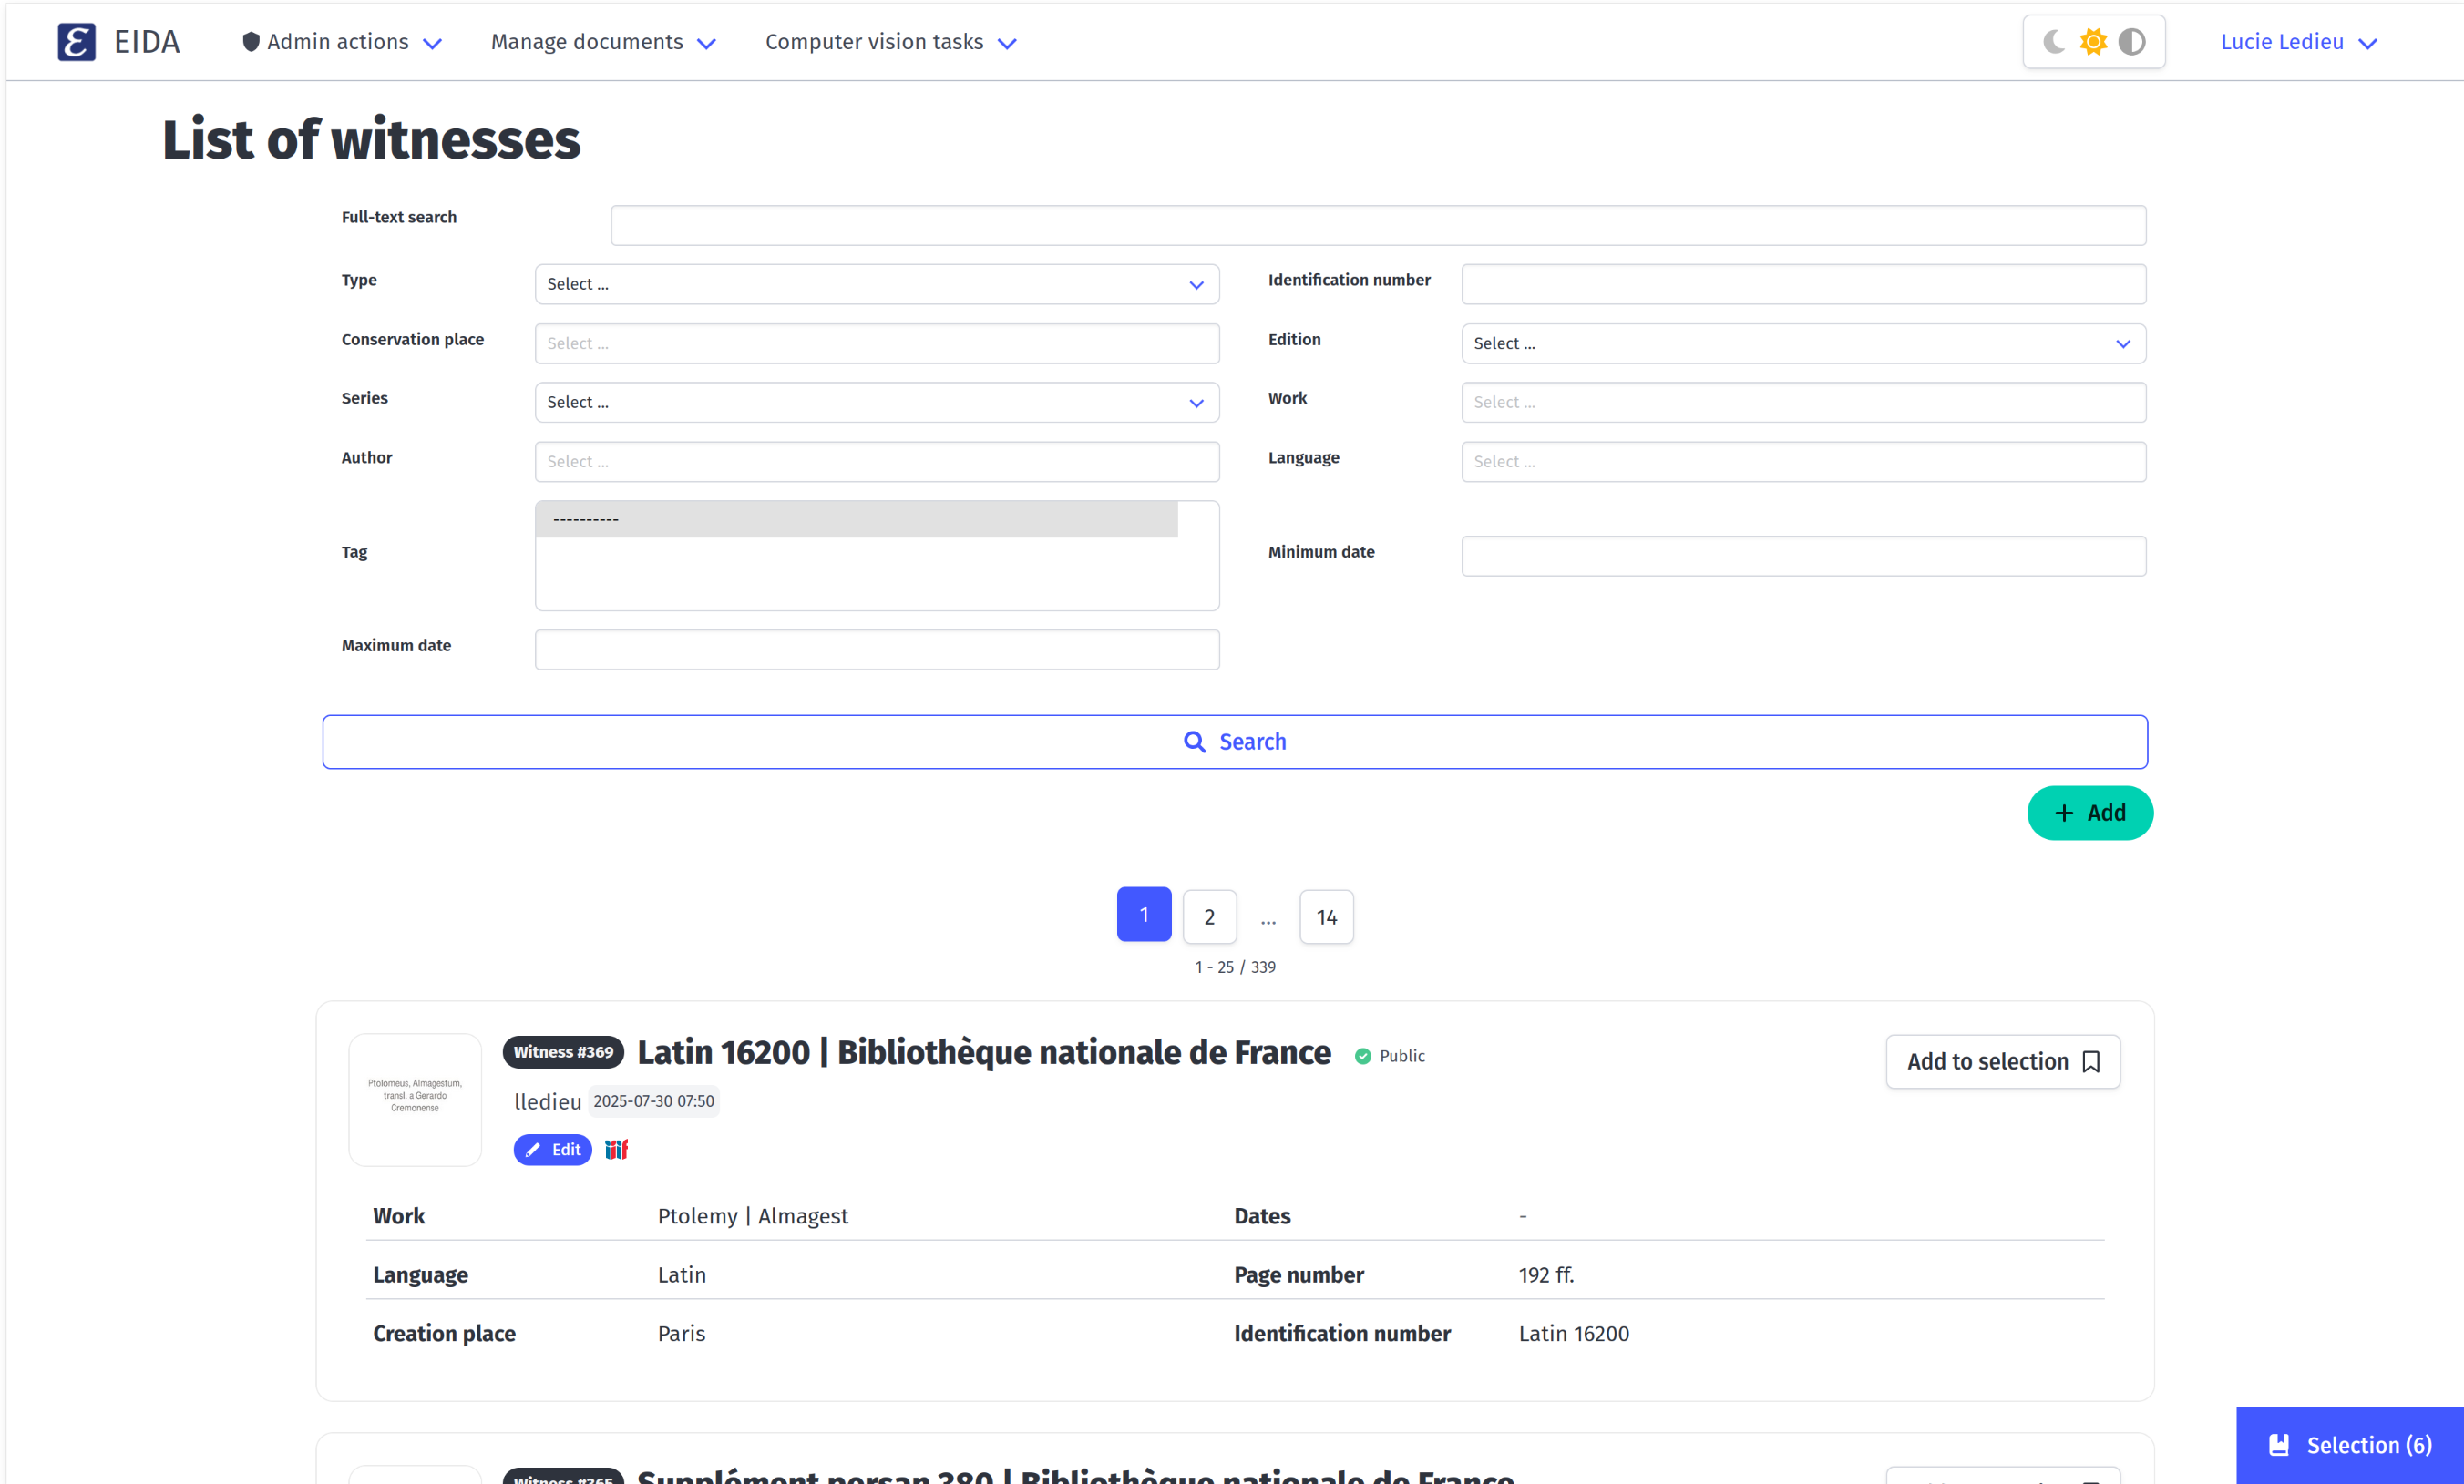
\includegraphics[width=0.8\textwidth]{images/list_witnesses.png}
	\caption{Capture d'écran de l'interface de consultation des différents \textit{witnesses} sur \gls{eida}}
	\label{fig:apercu_witnesses}
\end{figure}

Les différents \textit{witnesses} peuvent être organisés en sous-ensembles cohérents. Par exemple, nous pouvons réunir tous les volumes d'une même édition disponibles dans différentes institutions. Il est d'ailleurs aussi possible de réunir plusieurs \textit{witnesses} en un \textit{work} quand il s'agit de la même œuvre.

Pour créer sa propre collection de \textit{witnesses}, nous avons la possibilité de créer des \textit{document sets} en cliquant sur \og Add to selection \fg. Cette fonctionnalité est utile notamment lorsque nous voulons lancer un traitement pour plusieurs \textit{witnesses} à la fois.

\subsection{L'extraction des regions}

AIKON propose une fonctionnalité permettant d'extraire des \textit{regions}. Dans le cas d'\gls{eida}, il s'agit des diagrammes. Cette action peut se faire de manière manuelle, notamment lors de l'entraînement de l'algorithme ou lorsque ce dernier fait une erreur. 

\subsubsection{L'annotation manuelle avec Mirador}

Pour annoter de manière manuelle les \textit{regions} d'un \textit{witness}, il faut se servir de Mirador\footcite{MiradorHome}, un outil \textit{open-source} d'annotation d'image. Afin d'y accéder, il faut se rendre sur la page d'un des \textit{witnesses} et choisir \og \textit{Manually annotate}\fg. Pour définir une \textit{region}, il faut l'encadrer en utilisant le carré ou le cercle mis à disposition dans la barre de fonctionnalité.

\begin{figure}[H]
	\centering
	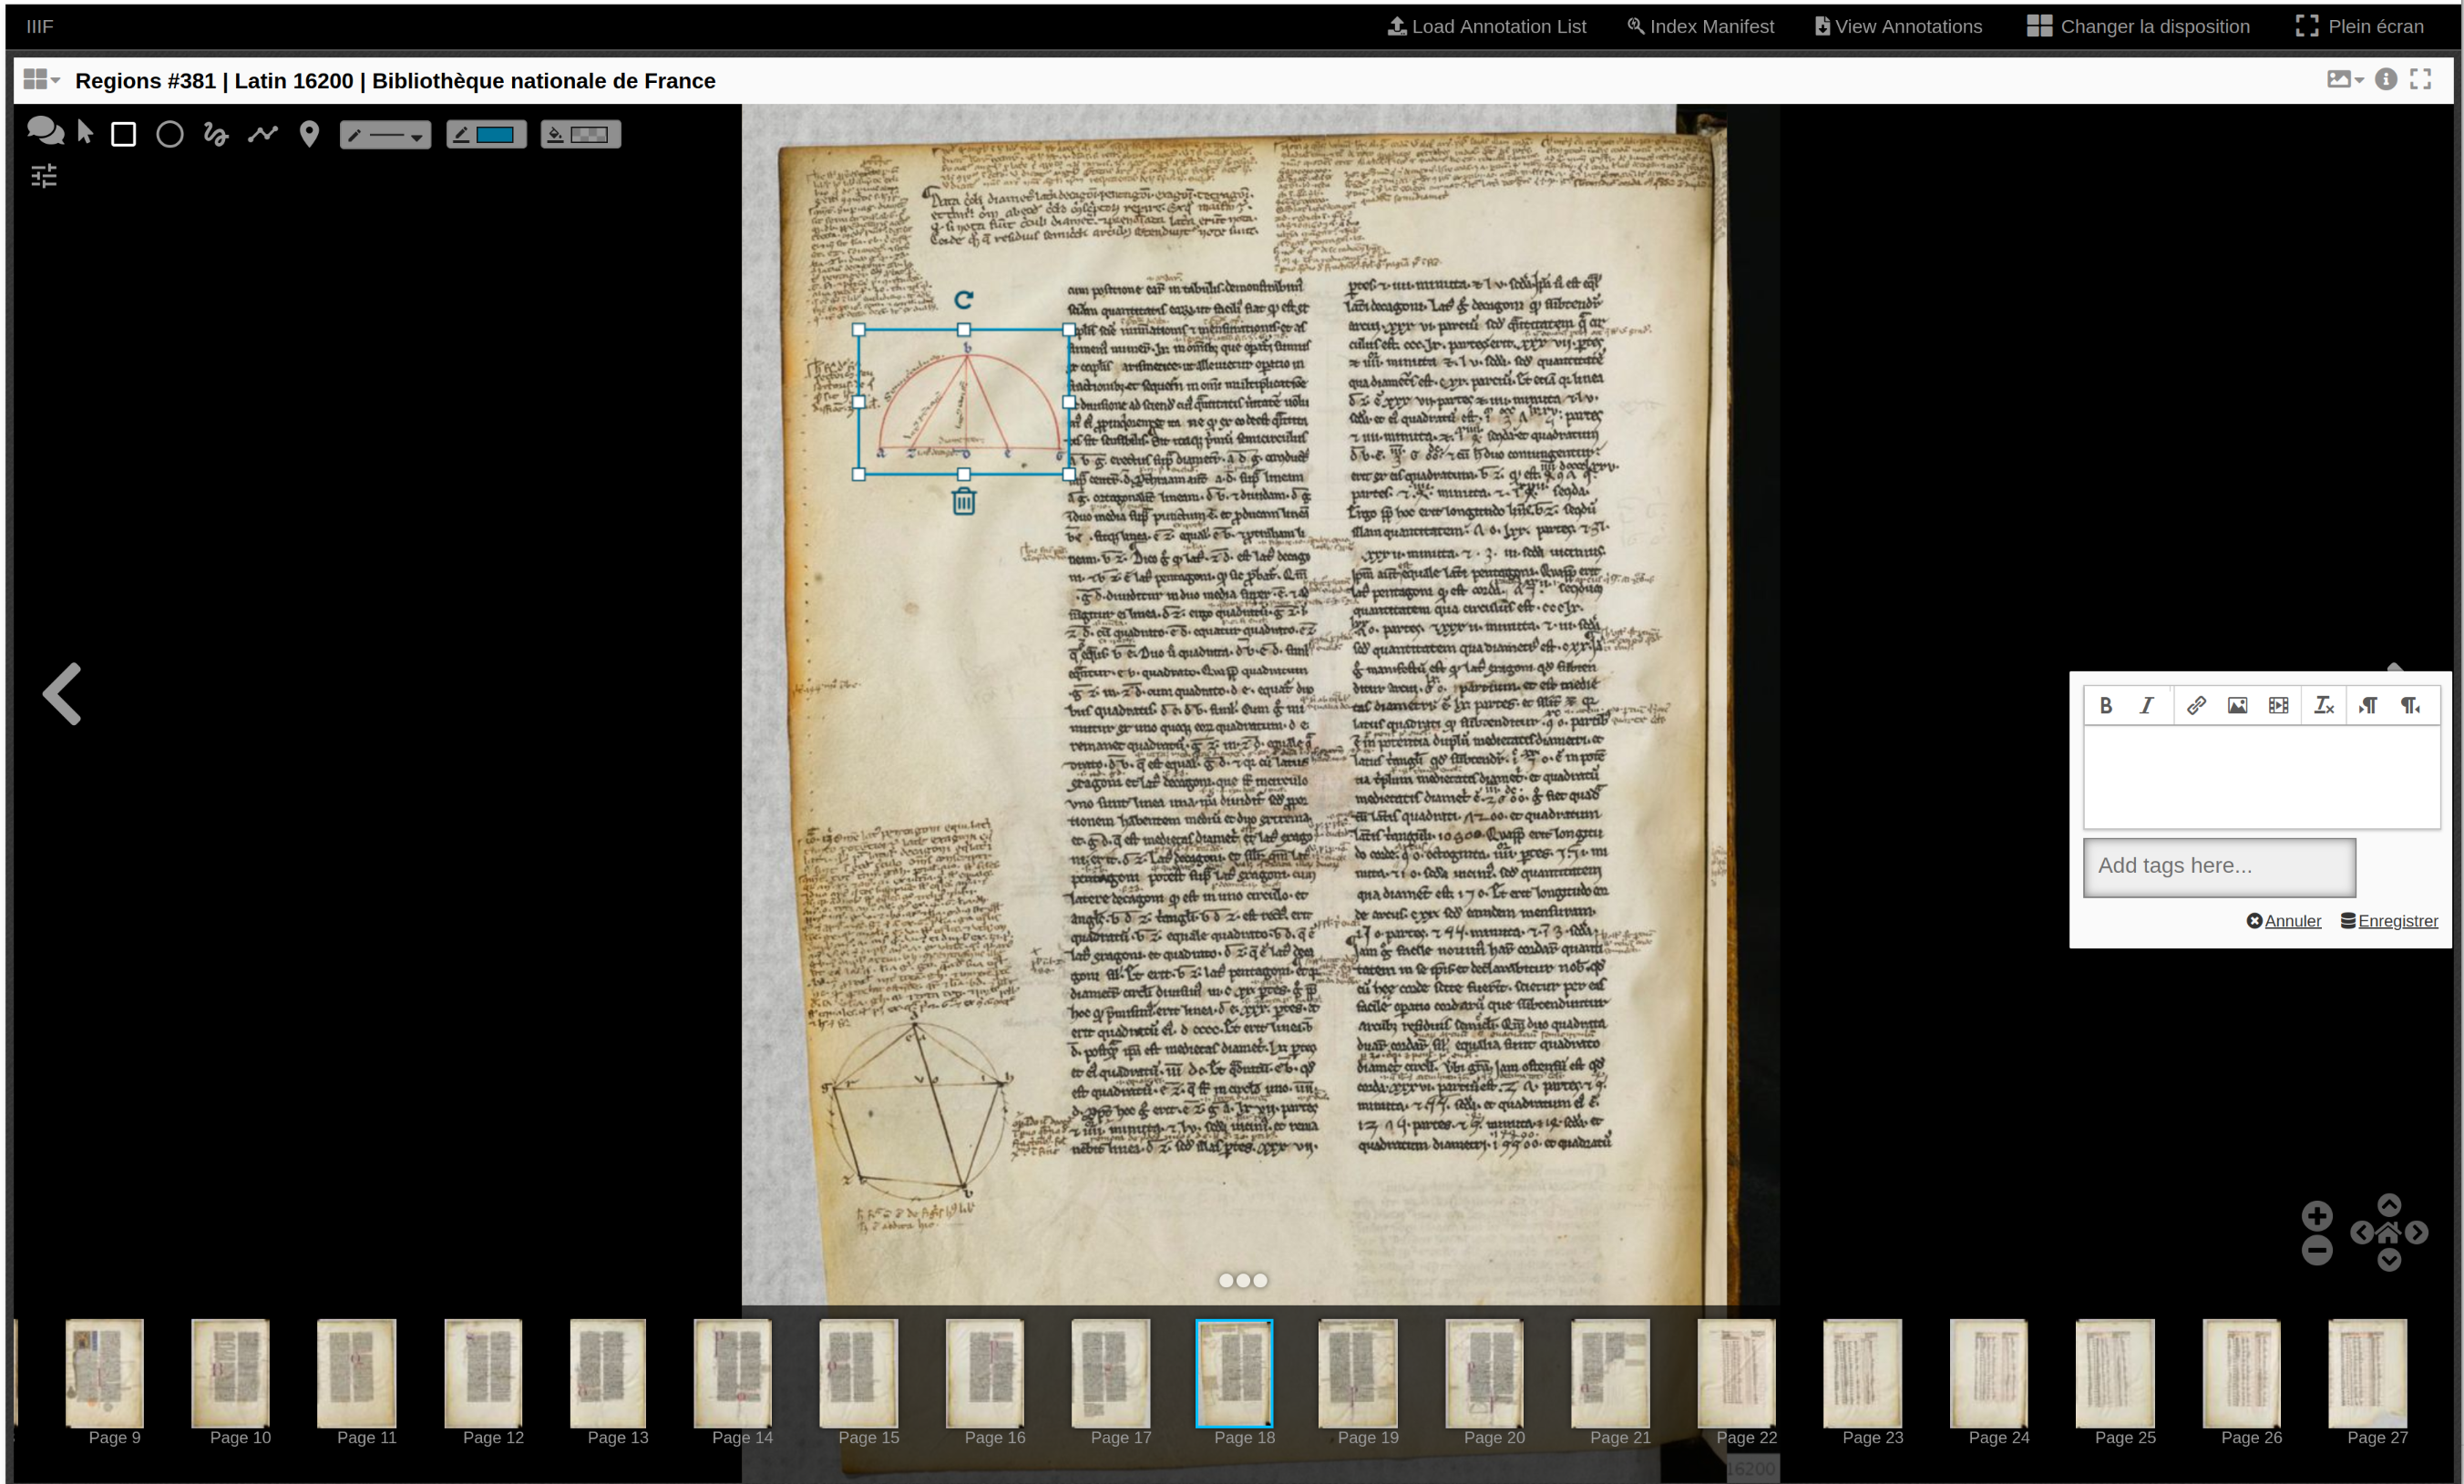
\includegraphics[width=0.8\textwidth]{images/capture_ecran_mirador.png}
	\caption{Aperçu de l'outil Mirador et de ses fonctionnalités}
	\label{fig:apercu_mirador}
\end{figure}


\subsubsection{L'extraction automatique des regions}

Annoter manuellement chaque \textit{region} est chronophage. Heureusement, il existe des algorithmes pour réaliser une extraction automatique de toutes les \textit{regions} d'un \textit{witness}. 
Pour faire cette opération, il faut se rendre sur la page d'un des \textit{witnesses} puis choisir \og textit{Automatic region extraction} \fg. Comme nous l'avons vu précédemment, il existe plusieurs algorithmes. Pour les diagrammes astronomiques, le plus approprié est \og \textit{Diagram extraction (YOLO model fine-tuned on historical diagrams)}\fg.


\begin{figure}[h]
	\centering
	\begin{subfigure}{0.48\linewidth}
		\centering
		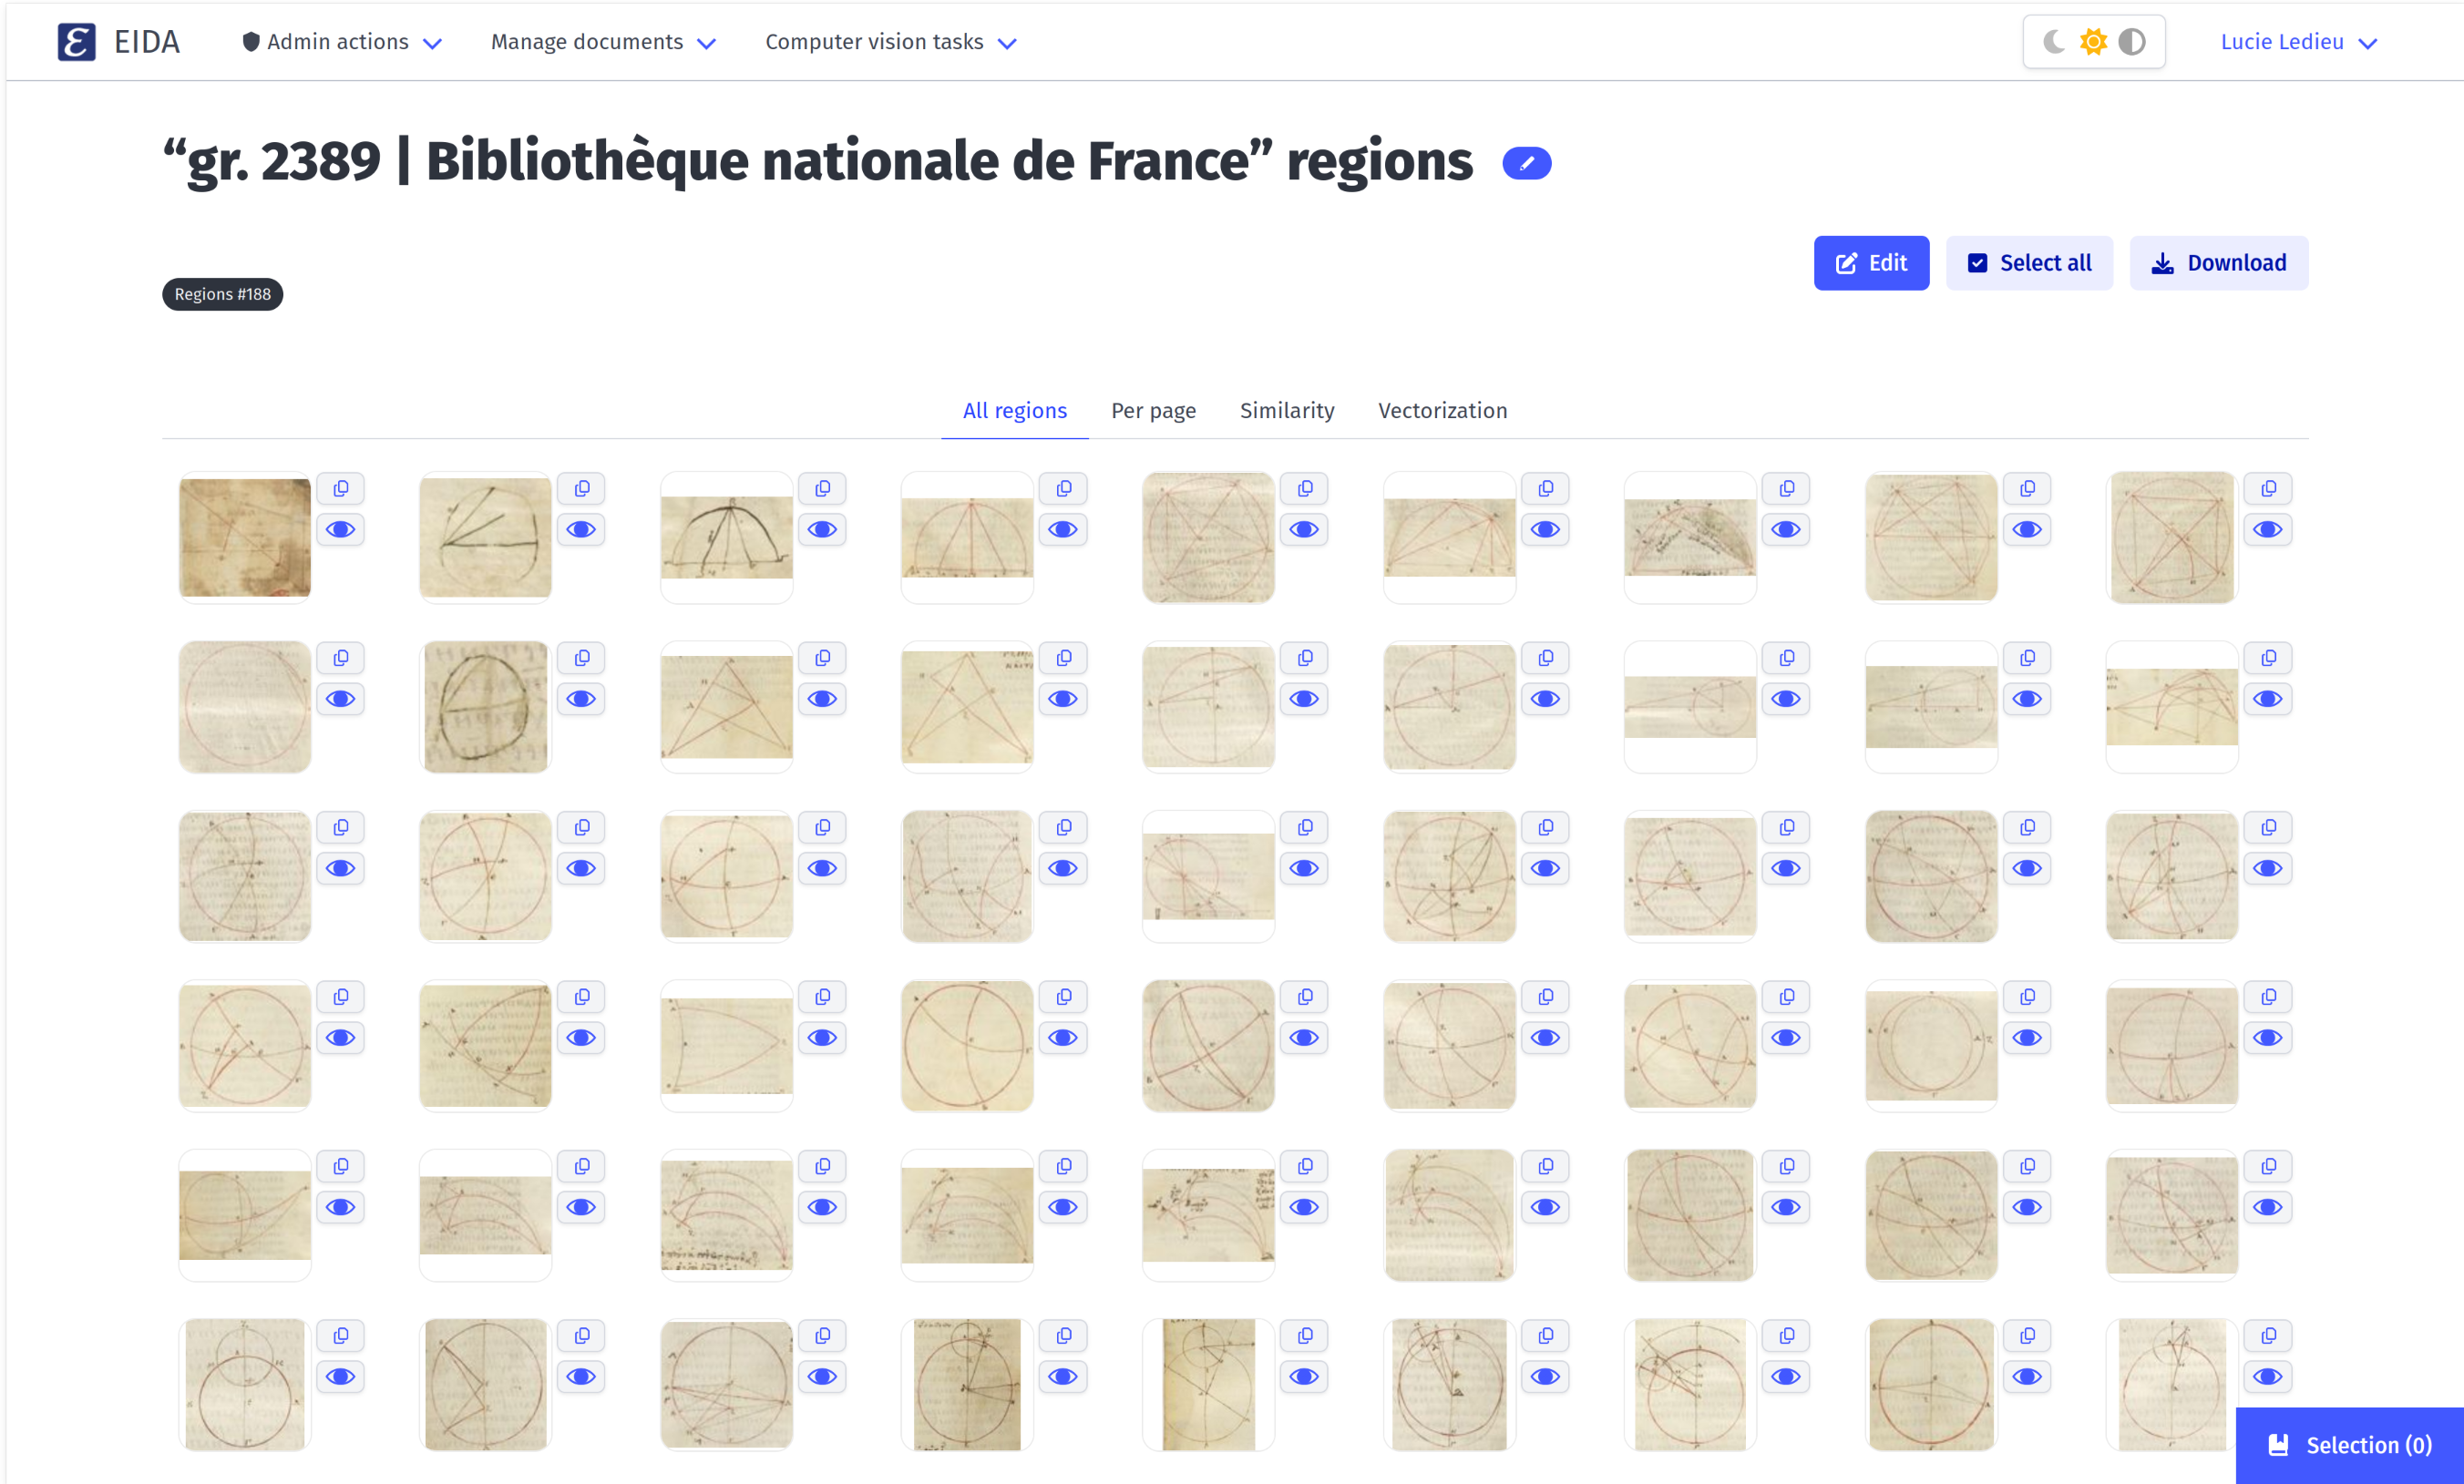
\includegraphics[width=\linewidth]{images/regions_par_witness.png}
	\end{subfigure}
	\hfill
	\begin{subfigure}{0.48\linewidth}
		\centering
		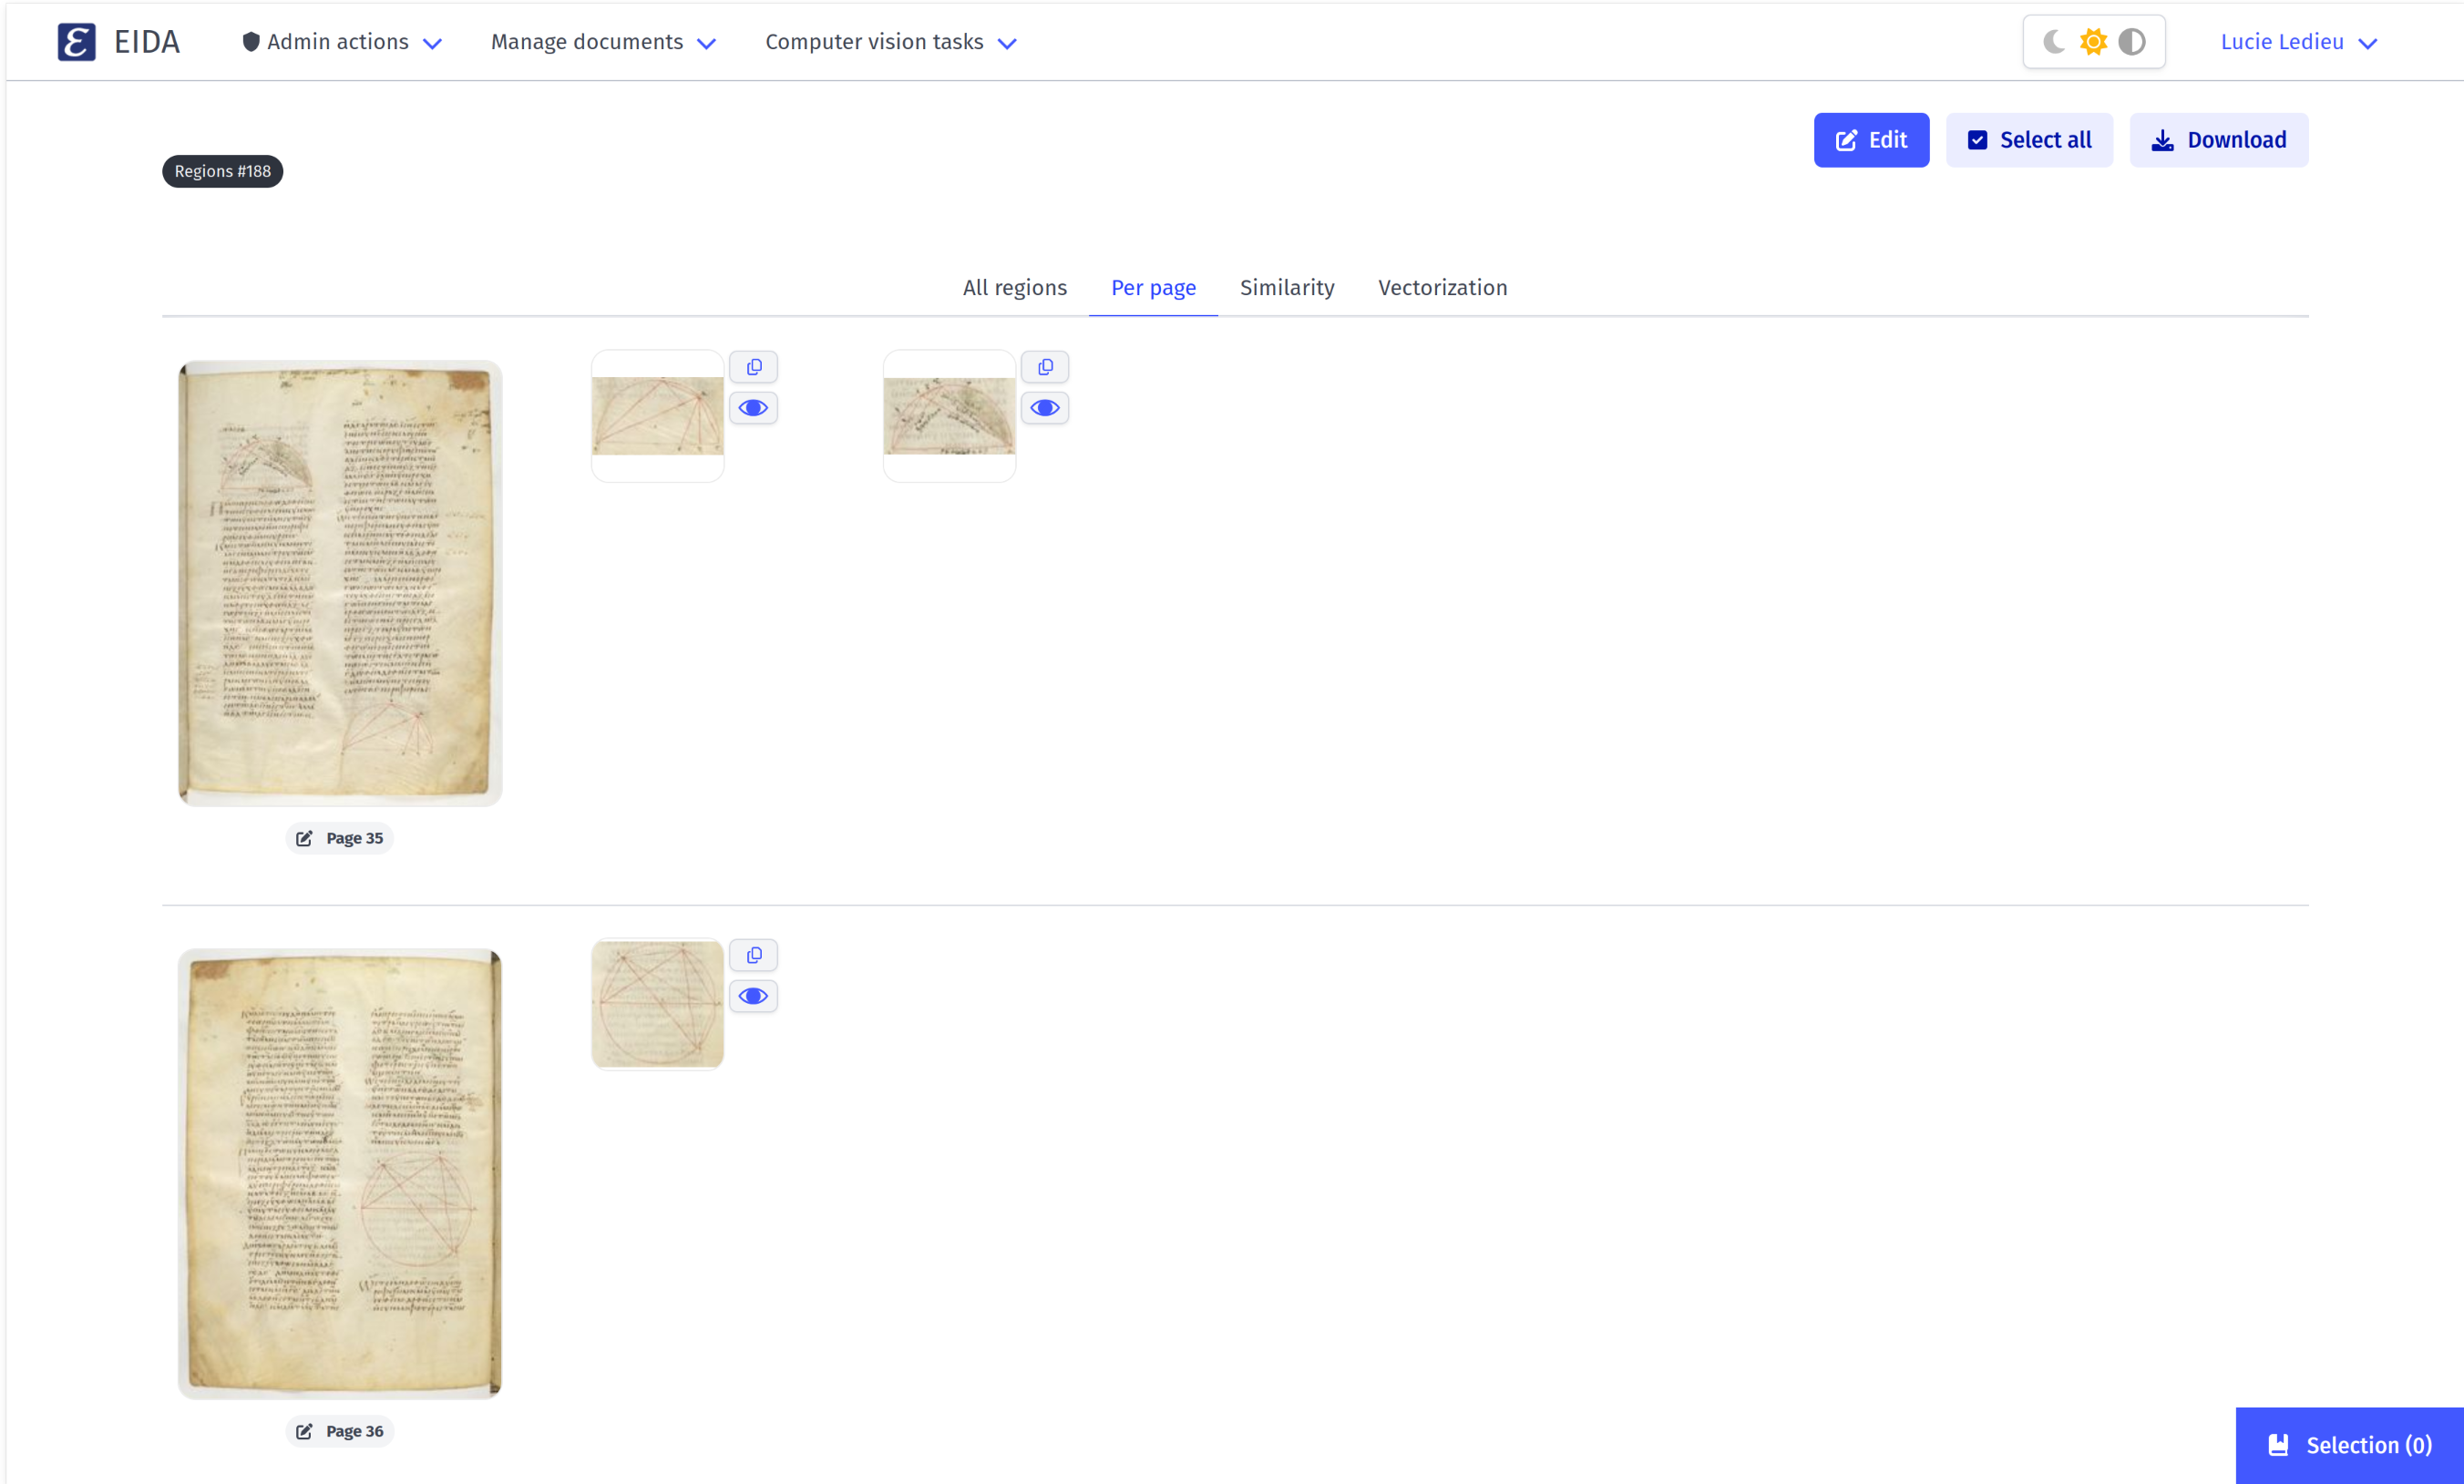
\includegraphics[width=\linewidth]{images/regions_par_page.png}
	\end{subfigure}
	\caption{\textit{Regions} extraites par \textit{witness} et par page}
	\label{fig:regions_extraction}
\end{figure}


Une fois le traitement terminé, nous pouvons visualiser les différents diagrammes extraits soit dans le \textit{witness} entier, soit page par page.

En cas d'erreur de l'algorithme, il est évidemment possible d'y remédier via Mirador.

\subsection{La constitution de correspondances entre les regions}

\subsubsection{La reconnaissance automatique et le calcul du score de similarités}

La plateforme AIKON propose une fonctionnalité de reconnaissance automatique de similarités couplée à la possibilité de calculer un score de similarité en chaque \textit{region} similaire. 

Pour commencer, il faut sélectionner les différents \textit{witnesses} à comparer dans un \textit{document set}. Ensuite, nous devons nous rendre dans l'onglet \og \textit{Computer vision tasks} \fg puis cliquer sur \og \textit{Add new treatment} \fg et choisir \og \textit{Compute similarity score} \fg dans \og \textit{Task type} \fg. Il est aussi possible de faire une extraction automatique de \textit{regions} dans plusieurs \textit{witnesses} au même endroit. Pour extraire des diagrammes, la meilleure solution est d'utiliser l'algorithme \textit{SegSwap} que nous avions cité précédemment. 

\begin{figure}[H]
	\centering
	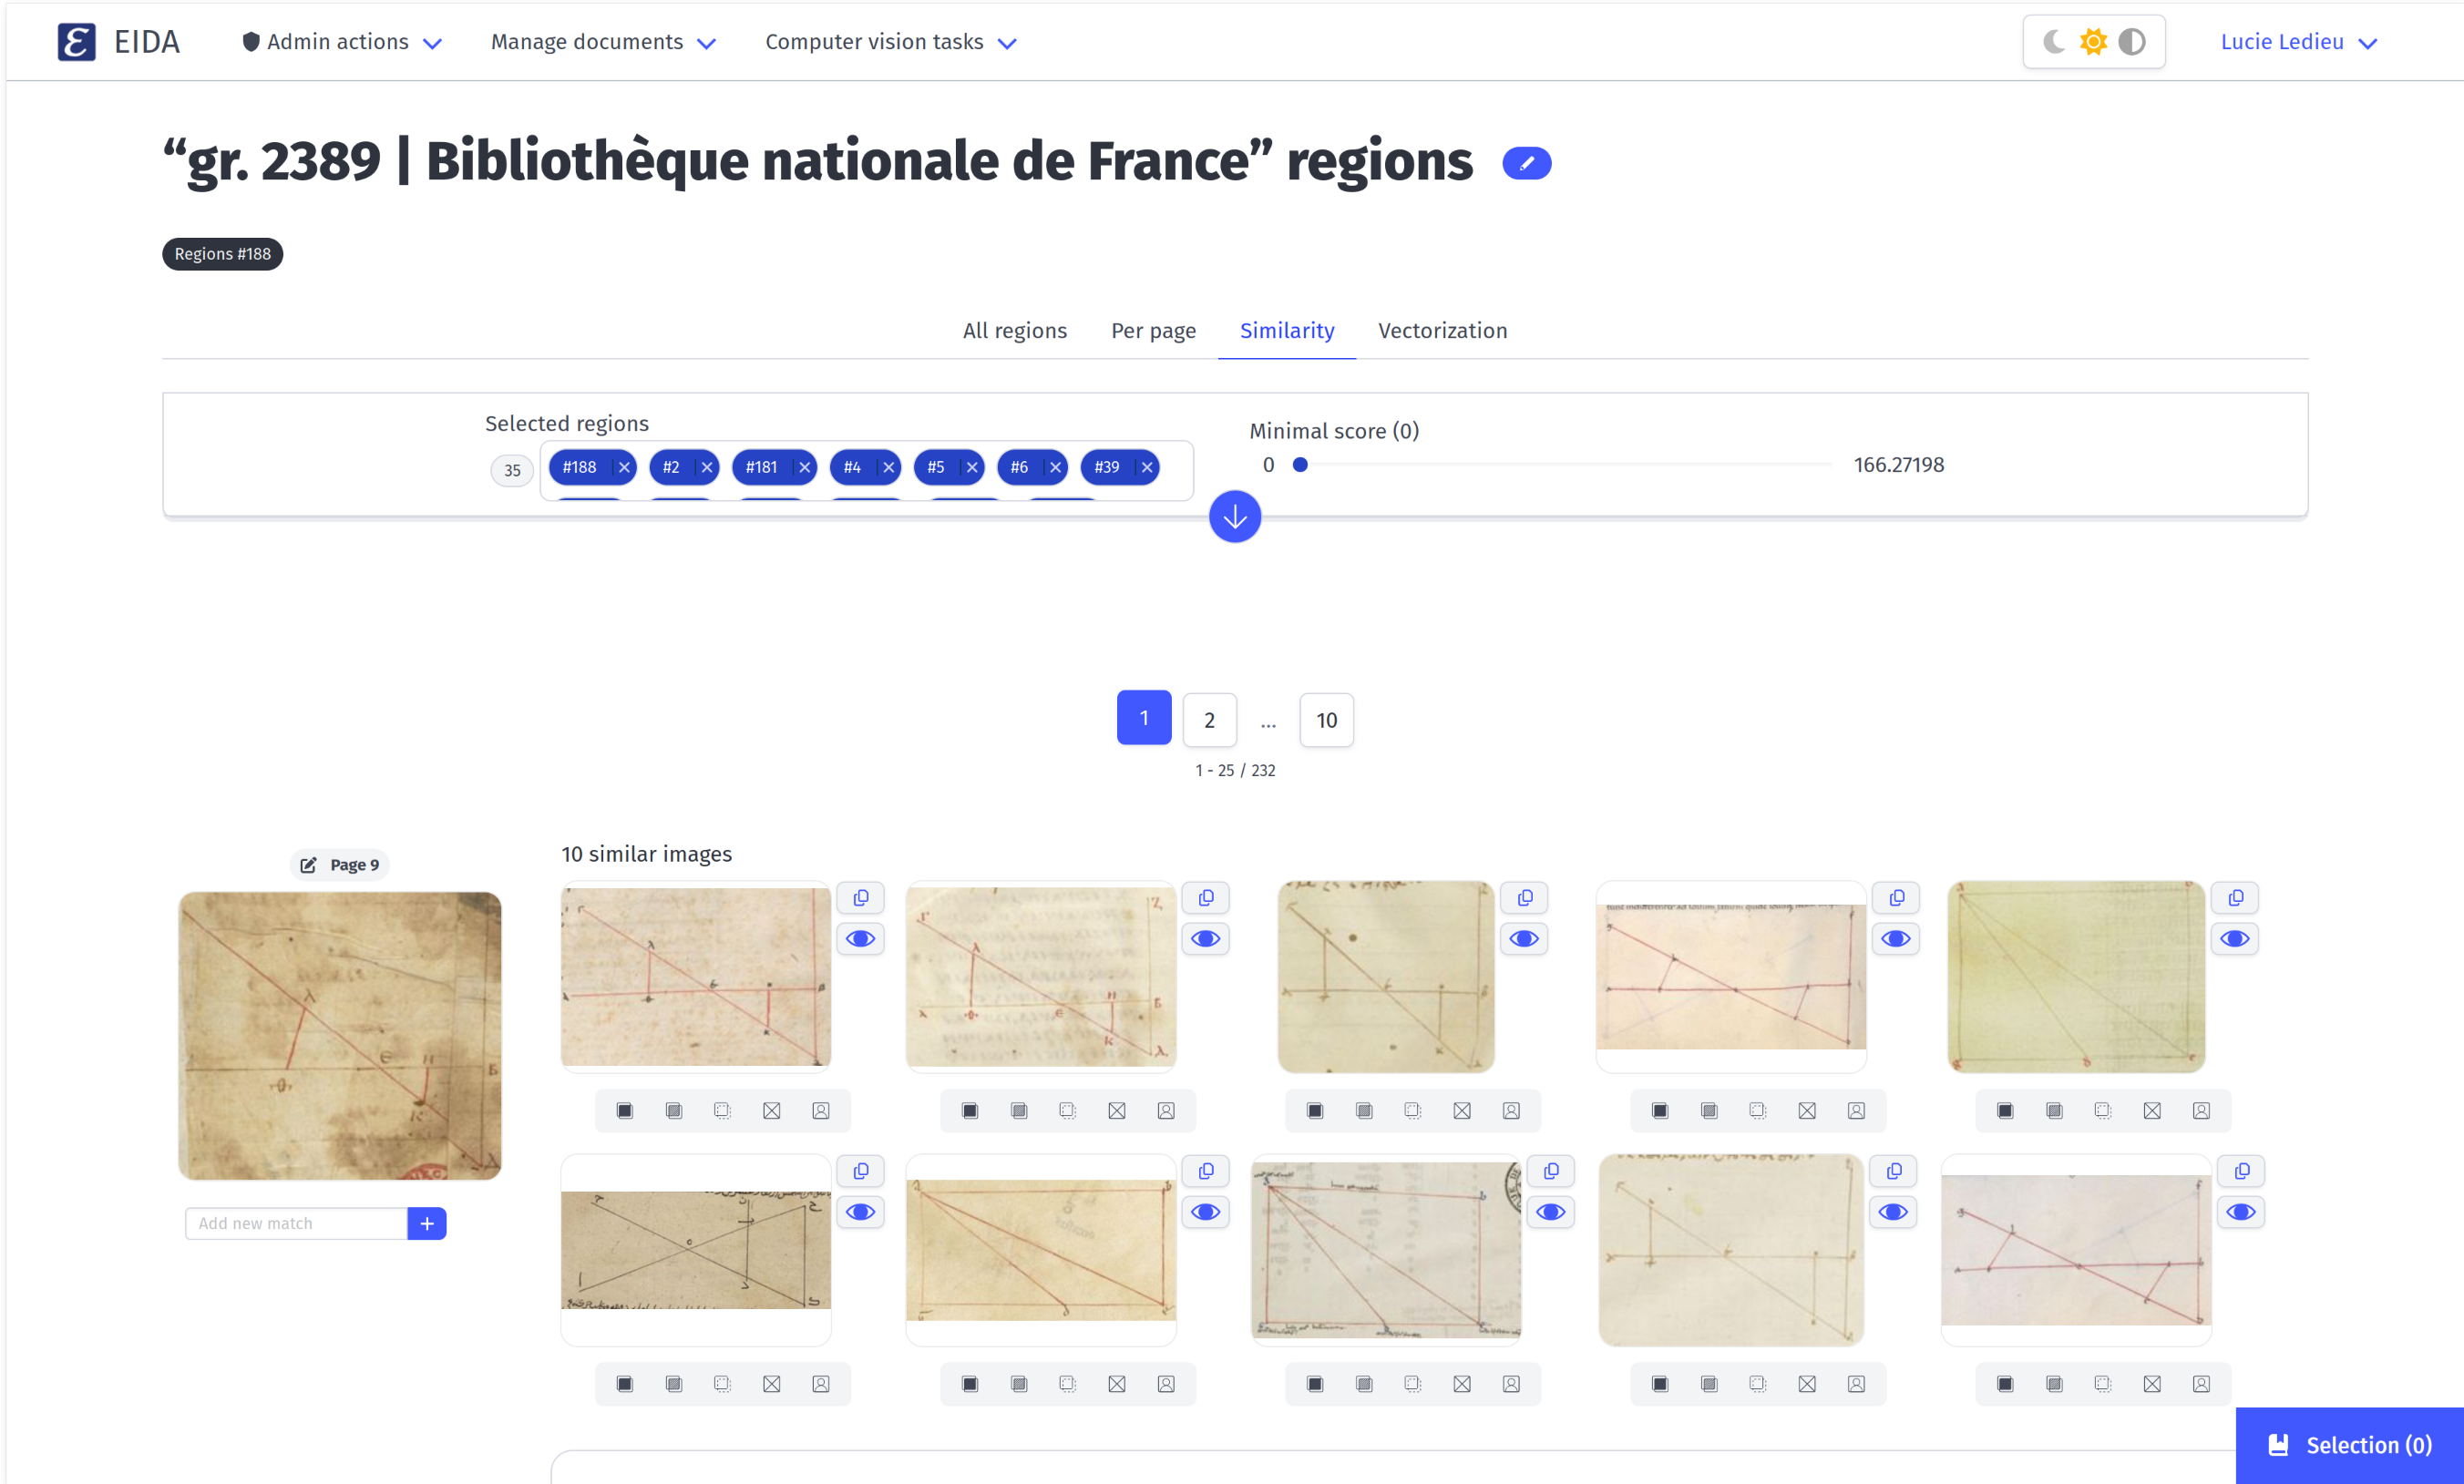
\includegraphics[width=0.8\textwidth]{images/similarities.png}
	\caption{Aperçu des différentes \textit{regions} similaires dans un \textit{witness}}
	\label{fig:apercu_similarites}
\end{figure}

Une fois le traitement réalisé, nous pouvons observer les résultats en retournant sur un des \textit{witnesses}. 
IL est possible de les filtrer grâce au formulaire en haut qui propose de choisir quels \textit{witnesses} nous voulons comparer. IL y a également un curseur pour choisir le score de similarité minimal.

\subsubsection{L'annotation des résultats}


Même si l'objectif final serait de créer des outils d'intelligence artificielle qui n'ont pas besoin d'être annotés au préalable, nous sommes à une étape du projet où il est encore nécessaire de le faire pour entraîner les algorithmes.

\begin{figure}[H]
	\centering
	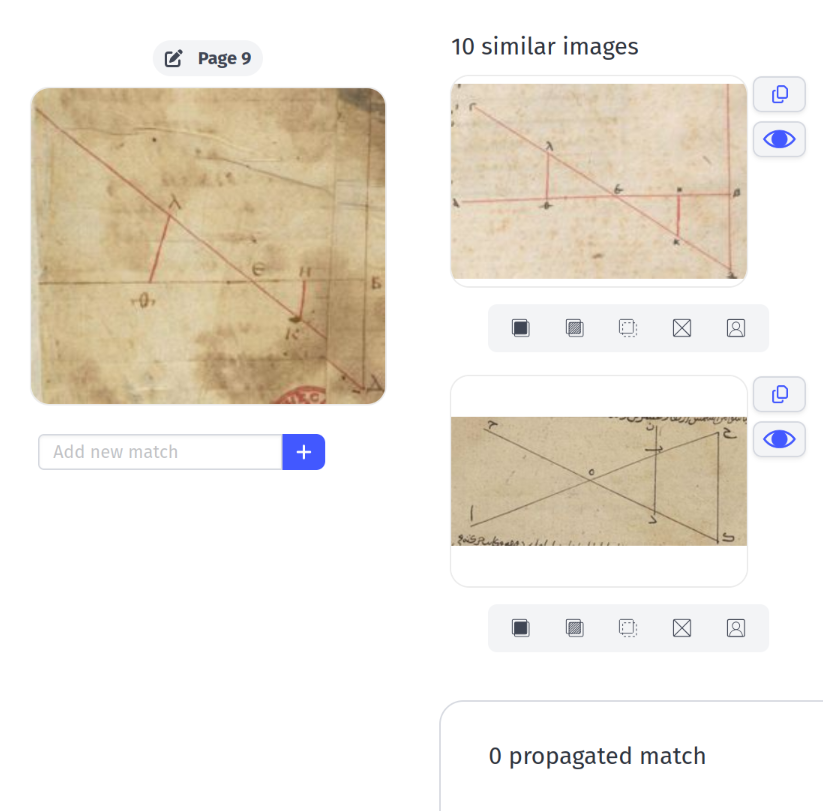
\includegraphics[width=0.8\textwidth]{images/annotation_similarities.png}
	\caption{Aperçu de l'interface d'annotation des similarités}
	\label{fig:annotations_similarites}
\end{figure}

Pour annoter les différentes \textit{regions}, il y a un petit panneau en dessous de chacune d'entre-elles avec plusieurs cases qui représentent le type d'annotation : 
\begin{enumerate}
	\item \textit{Exact match} : Les deux \textit{regions} sont parfaitement similaires.
	\item \textit{Partial match} : Les deux \textit{regions} sont un peu différentes.
	\item \textit{Semantic match} : Les deux \textit{regions} sont différentes physiquement mais d'un point de vue théorique elles représentent un même concept ou signification.
	\item \textit{No match} : les deux \textit{regions} ne sont pas du tout similaires.
\end{enumerate} 


En ce qui concerne le projet \gls{eida}, l'objectif final serait de développer une interface publique sur le même modèle que celle du projet \gls{dishas}.

\begin{figure}[H]
	\centering
	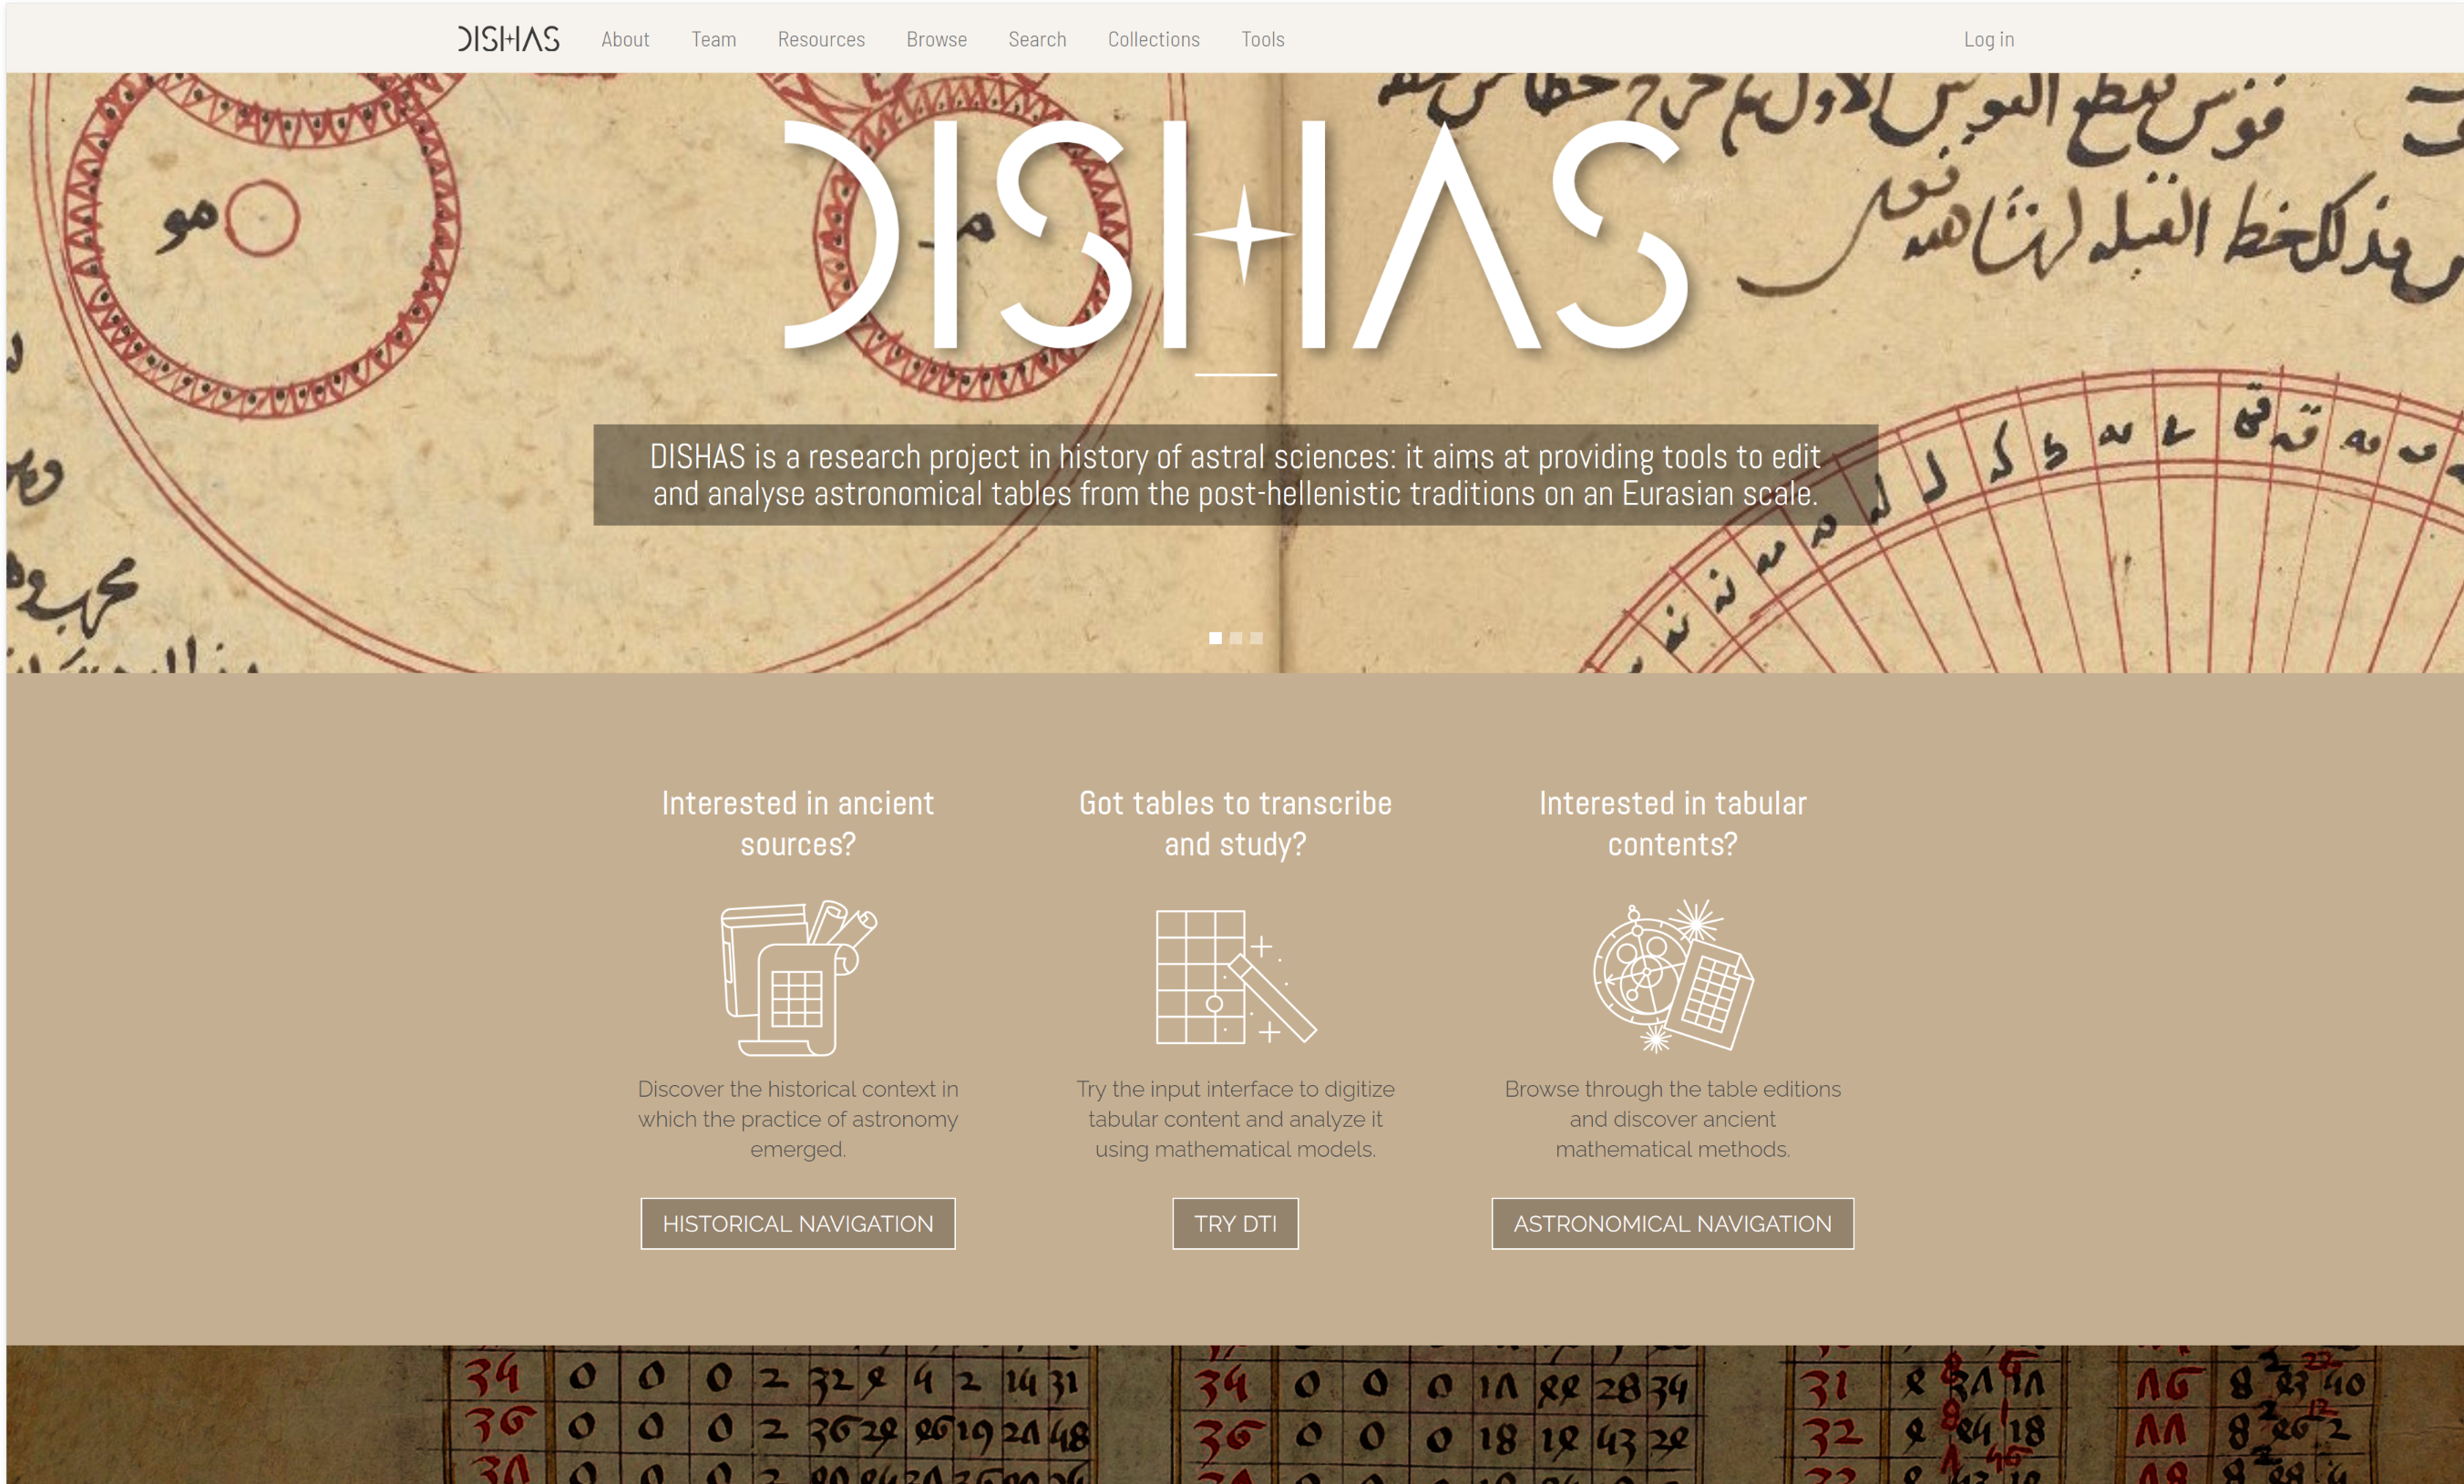
\includegraphics[width=1\textwidth]{images/dishas.png}
	\caption{Capture d'écran de l'interface publique de \gls{dishas}}
	\label{fig:dishas-interface}
\end{figure}

L'objectif principal d'une interface publique ou \textit{front-office} est de mettre à disposition des utilisateurs les différents outils développés au cours du projet ainsi que les résultats obtenus. Lors de sa création, le dialogue avec les chercheurs est primordial. En effet, il doit y avoir un \og fil conducteur \fg suivant les différentes hypothèses scientifiques ayant orienté leur réflexion dans la navigation entre les différentes pages. Les données doivent être contextualisées dans leur corpus ainsi que dans le projet en général\footcite{albouyMediationDonneesRecherche2019}.Dans ce contexte, il est essentiel de réaliser des visualisations afin de les rendre accessible, de mieux les comprendre et de les explorer de manière interactive. 